%-------------------------------------------------------------------------------
\section{String signal morphing/shape studies}
\label{sec:StrMorphShapeStudies} 
%%\addtocontents{toc}{\protect\setcounter{tocdepth}{0}} 

This appendix focusses on the shape studies performed with the string signal MC samples. The morphing part is also discussed.

%-------------------------------------------------------------------------------

\subsection{Signal morphing}
\label{subsec:StrMorphShapeStudies:SigMorph}
Due to the availability of limited computing resources as well as time crunch, MC signal shapes can be generated for a limited number of masses only. In case there is a need for more MC signal shapes, it's worth using the interpolation between the already generated signal shapes to obtain various intermediate signal shapes. This procedure is called signal morphing. First, the generated MC signal shapes are fit successfully using suitable functions. Following the fits, all the fit parameters become functions of mass. Then, the corresponding fit parameters from different signal shapes are fit with the cubic splines. Afterwards, applying the interpolation technique, the intermediate  signal shapes are created by evaluating the spline fits at the desired mass points. 

~~~~~~~~ Five string signal MC samples have been generated for the dijet q/g tagged analysis. One could use the splines from the fits of these samples, but there seems to be no need for further signal morphing as the generated samples sufficiently cater to the requirement.


%-------------------------------------------------------------------------------

\subsection{Initial shape studies}
\label{subsec:StrMorphShapeStudies:InitShapStud}

The usual Gaussian+reverse-Landau (GrL) function does a fairly good job of fitting a wide variety of MC signals used in the high mass dijet searches. They work well for excited quark ($q^{*}$ ), $W$ and $Z$ signals. On the other hand, the string signals are a bit unusual in nature -- their mass does not peak around the mass scale ($M_{s}$) used during the generation. The motivation for string signal shape studies comes from this very unusual nature of the samples. 

~~~~~~~ The very first string signal shape studies had been carried out during the initial days of the analysis, when the selection cuts were not finalized. Therefore, the $m_{jj}$ distributions did not have any cuts applied to them and they also had a uniform bin-width of 100 GeV (Figure \ref{fig:InitStrmjj}). 

\begin{figure}[!htb]
  \centering
  \subfigure[$M_{s} = 7.0$ TeV.]{ 
  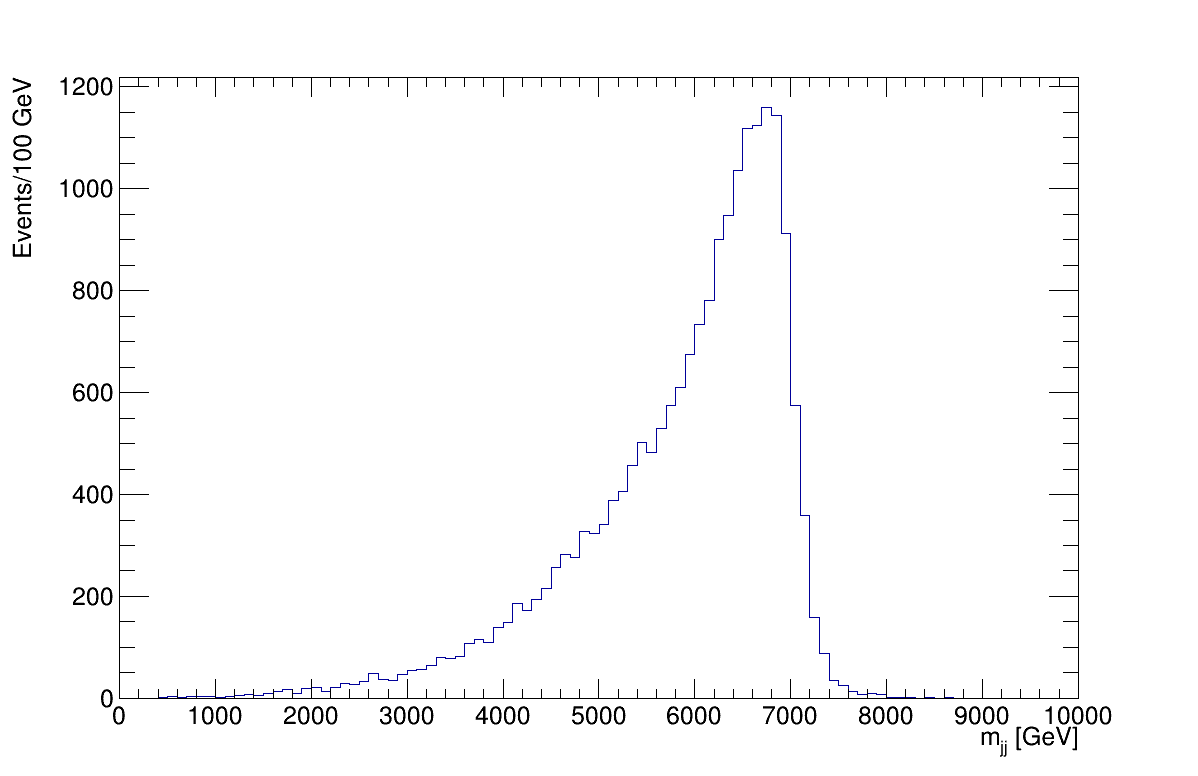
\includegraphics[width=0.45\textwidth]{figures/app-StrMorphShapeStudies/mjj_Old_string_ntuples_7TeV.png} }
  \subfigure[$M_{s} = 7.5$ TeV.]{  
  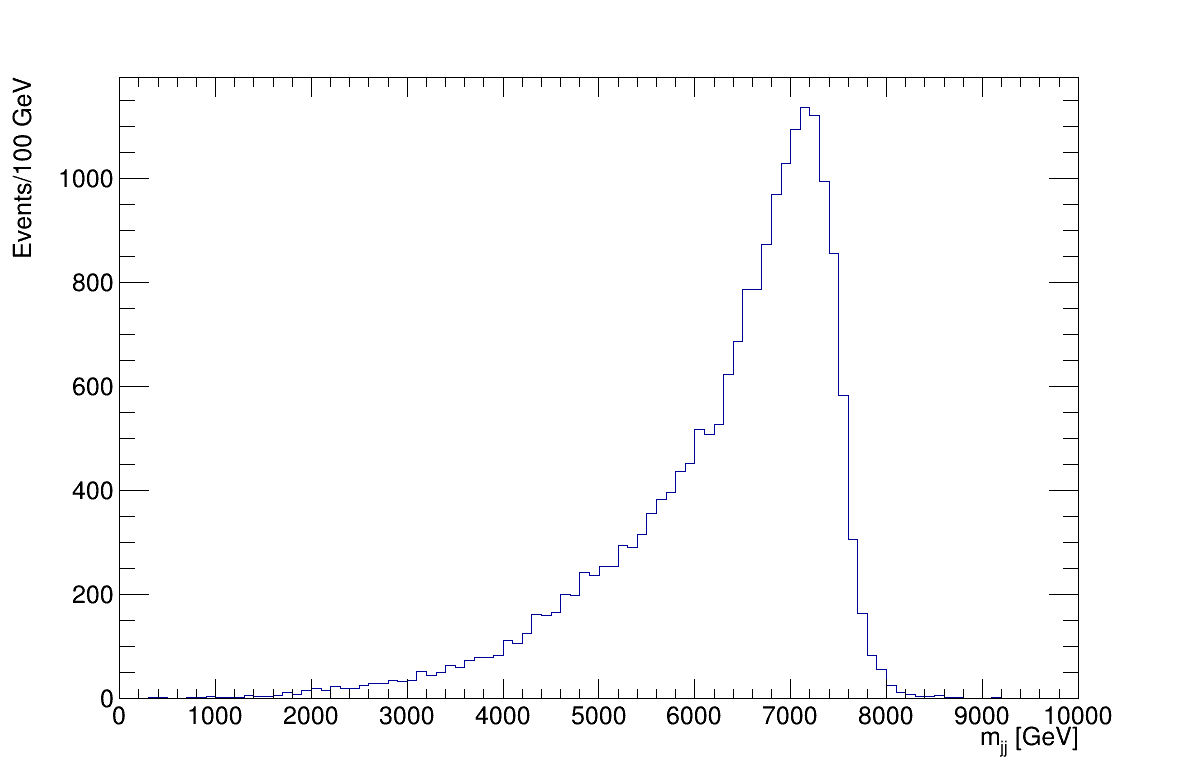
\includegraphics[width=0.45\textwidth]{figures/app-StrMorphShapeStudies/mjj_Old_string_ntuples_7p5TeV.png} }
  \subfigure[$M_{s} = 8.0$ TeV.]{
  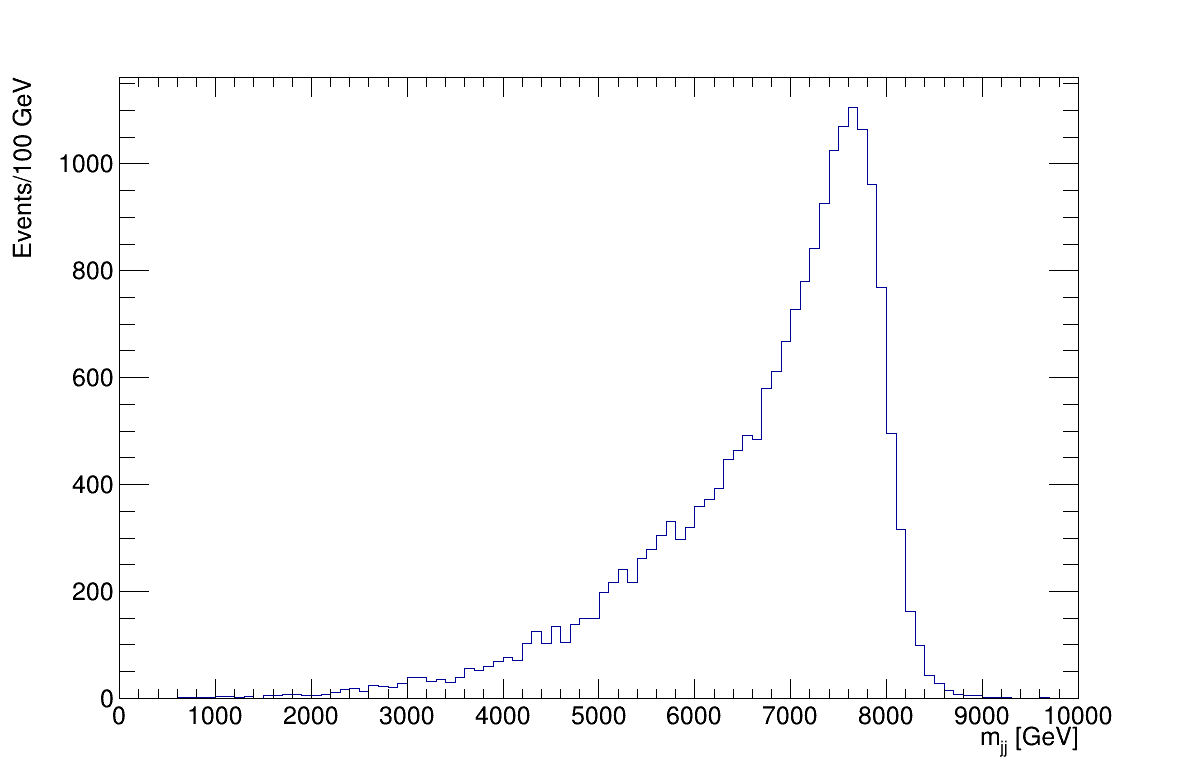
\includegraphics[width=0.45\textwidth]{figures/app-StrMorphShapeStudies/mjj_Old_string_ntuples_8TeV.png} }
  \subfigure[$M_{s} = 8.5$ TeV.]{                                                                 
  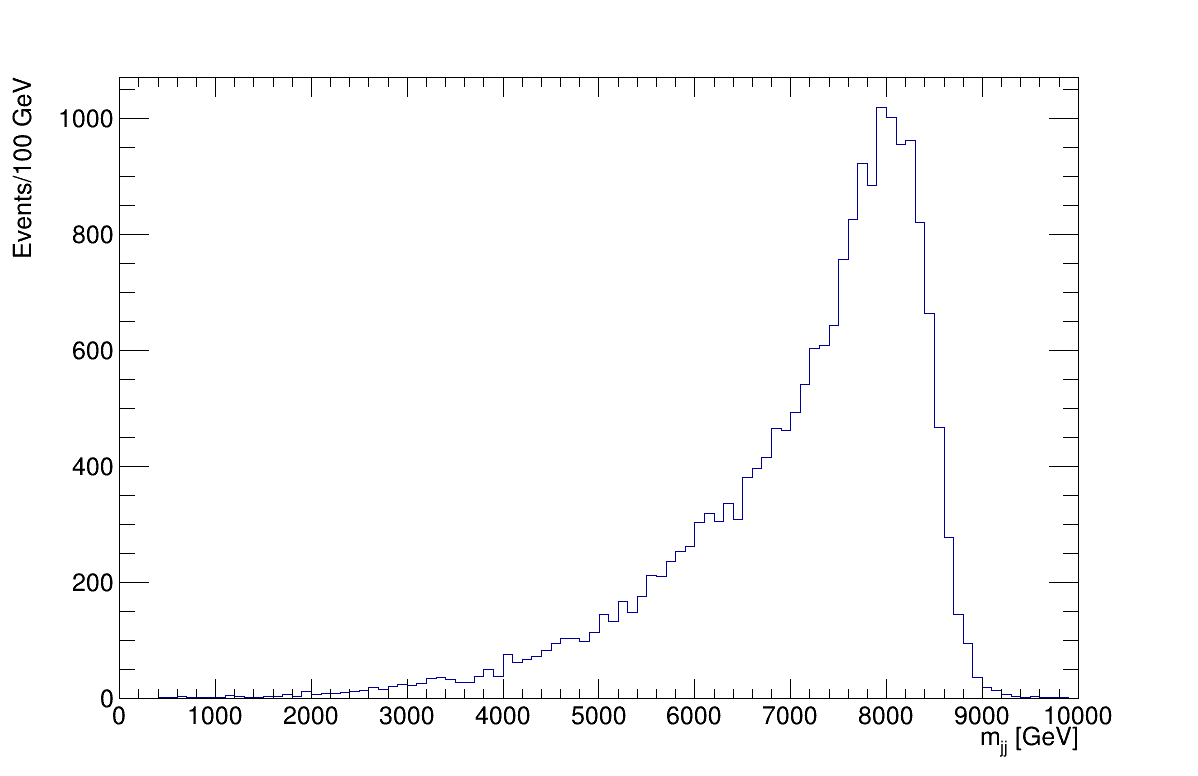
\includegraphics[width=0.45\textwidth]{figures/app-StrMorphShapeStudies/mjj_Old_string_ntuples_8p5TeV.png} }
  \subfigure[$M_{s} = 9.0$ TeV.]{
  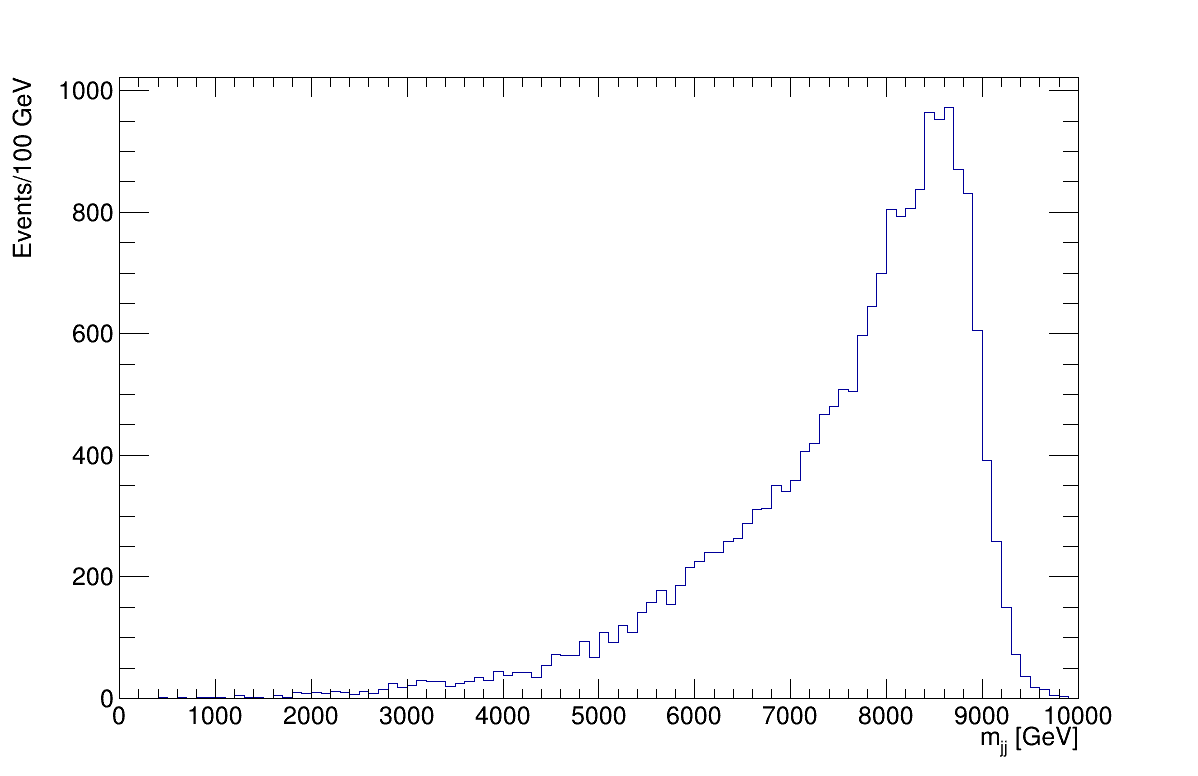
\includegraphics[width=0.45\textwidth]{figures/app-StrMorphShapeStudies/mjj_Old_string_ntuples_9TeV.png} }
  \caption{The string signal $m_{jj}$ shapes from the corresponding MC samples.}
  \label{fig:InitStrmjj}
\end{figure}



The list of functions that were considered to fit the $m_{jj}$ shapes are given below:

\begin{itemize}
    \item Crystal-Ball function (CB)
    \item Reverse-Landau (rL) 
    \item Comibation of a Gaussian and a reverse-Landau (GrL) 
    \item Convolution between a Gaussian and an exponential (GcE) $\rightarrow$ best results
    \item Combination of Planck and a Gaussian (PG) 
\end{itemize}   

The GcE is of the form

\begin{equation}
a~e^{-c~(-(x-b)-\frac{d^{2}c}{2})}[1+\mathrm{erf}(\frac{-(x-b)-d^{2}c}{d\sqrt{2}})]
\end{equation}

~ with $a$ -- amplitude, $b$ -- Gaussian mean (offset), $c$ -- lambda of exponential and $d$ -- Gaussian width (sigma).

~~~~~~ The expression for GrL (the conventional one) is 

\begin{equation} 
a ~[b ~ \mathrm{exp}(d(x-c)-e^{d(x-c)}) + (1-b) ~ \mathrm{exp}(-0.5 ~ (\frac{x-e}{f})^{2})] 
\end{equation}

~~ where $a$ -- relative normalization, $b$ -- fraction of reverse-Landau/Gaussian components, $c$ -- reverse-Landau mean (offset), $d$ -- reverse-Landau width (scale), $e$ -- Gaussian mean (offset), and $f$ -- Gaussian width (sigma).


   
\clearpage
 
The fits from GcE and GrL (the conventional one) are shown in Figures \ref{fig:InitGcEGrL-1} and \ref{fig:InitGcEGrL-2} for all string signal MC samples.  

\begin{figure}[!htb]
  \centering
  \subfigure[$M_{s} = 7.0$ TeV w/ GcE.]{
  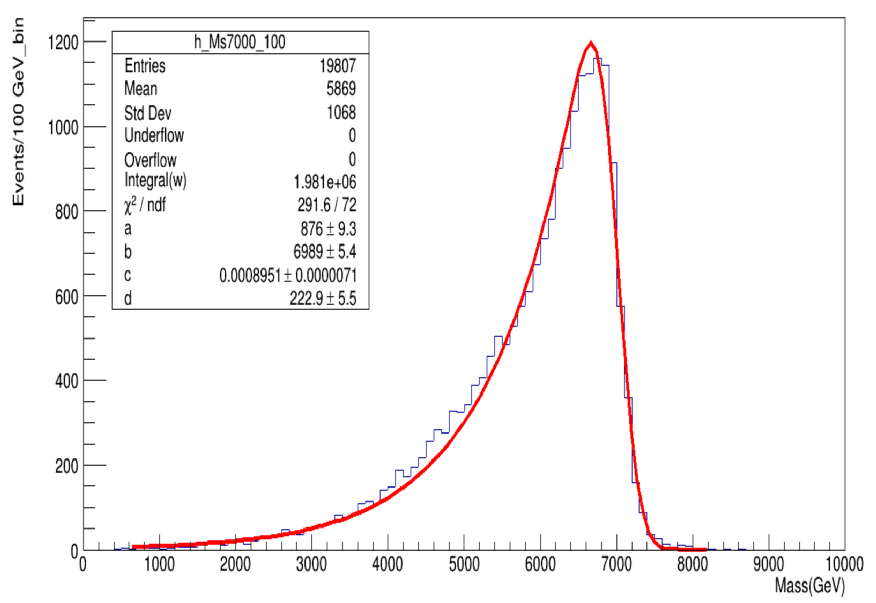
\includegraphics[width=0.45\textwidth]{figures/app-StrMorphShapeStudies/GcEFit_Old_ntuples_7TeV.png} }
  \subfigure[$M_{s} = 7.0$ TeV w/ GrL.]{
  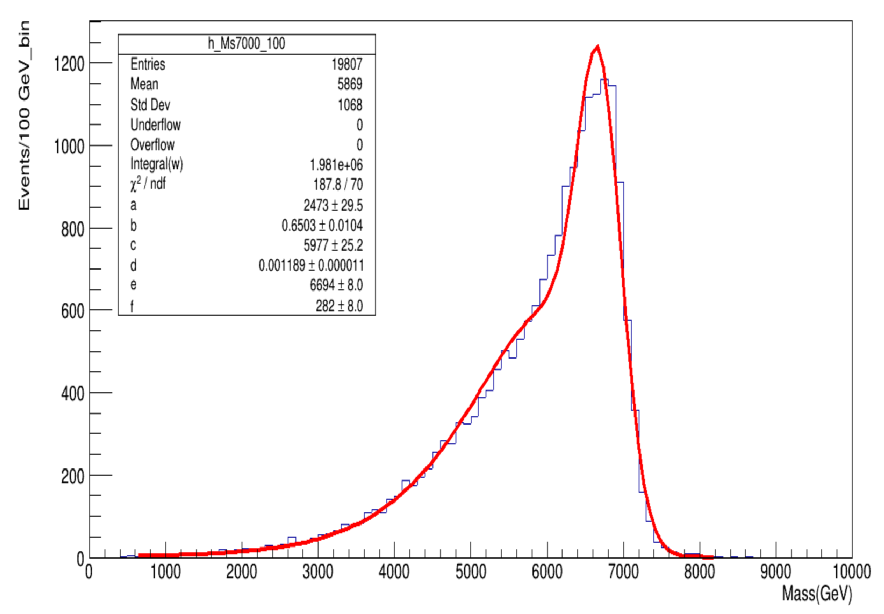
\includegraphics[width=0.45\textwidth]{figures/app-StrMorphShapeStudies/GrLFit_Old_ntuples_7TeV.png} }	
  \subfigure[$M_{s} = 7.5$ TeV w/ GcE.]{                                                                 
  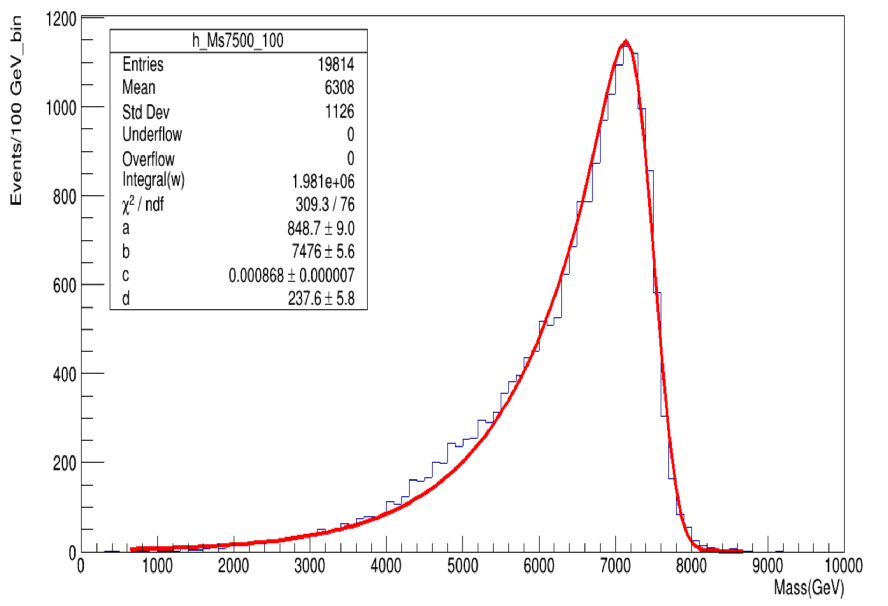
\includegraphics[width=0.45\textwidth]{figures/app-StrMorphShapeStudies/GcEFit_Old_ntuples_7p5TeV.png} }
  \subfigure[$M_{s} = 7.5$ TeV w/ GrL.]{
  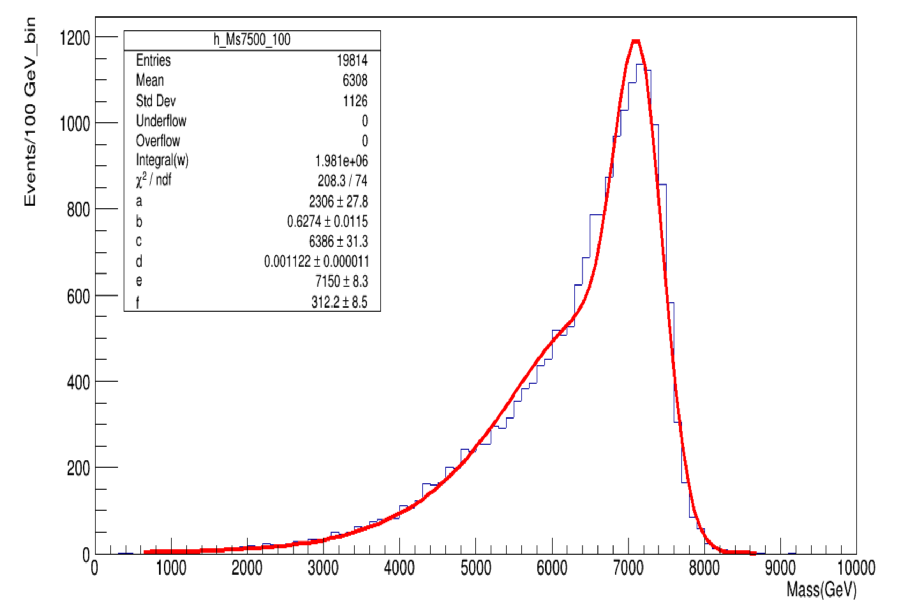
\includegraphics[width=0.45\textwidth]{figures/app-StrMorphShapeStudies/GrLFit_Old_ntuples_7p5TeV.png} }	
  \subfigure[$M_{s} = 8.0$ TeV w/ GcE.]{
  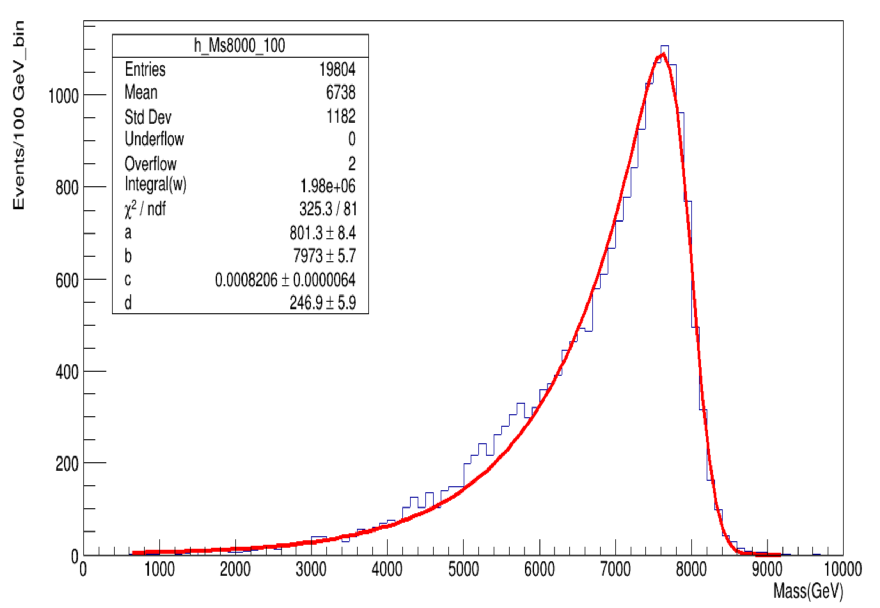
\includegraphics[width=0.45\textwidth]{figures/app-StrMorphShapeStudies/GcEFit_Old_ntuples_8TeV.png} }
  \subfigure[$M_{s} = 8.0$ TeV w/ GrL.]{
  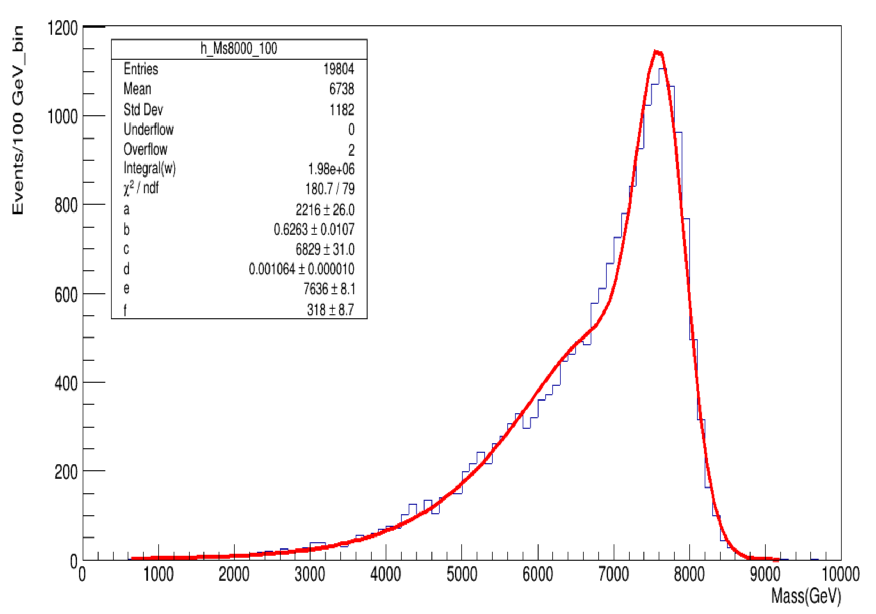
\includegraphics[width=0.45\textwidth]{figures/app-StrMorphShapeStudies/GrLFit_Old_ntuples_8TeV.png} }	
  \caption{The GcE and GrL fits on the string signal shapes for $M_{s} = 7.0,~7.5$ and $8.0$ TeV.}
  \label{fig:InitGcEGrL-1}
\end{figure}


\begin{figure}[!htb]
  \centering 
  \subfigure[$M_{s} = 8.5$ TeV w/ GcE.]{
  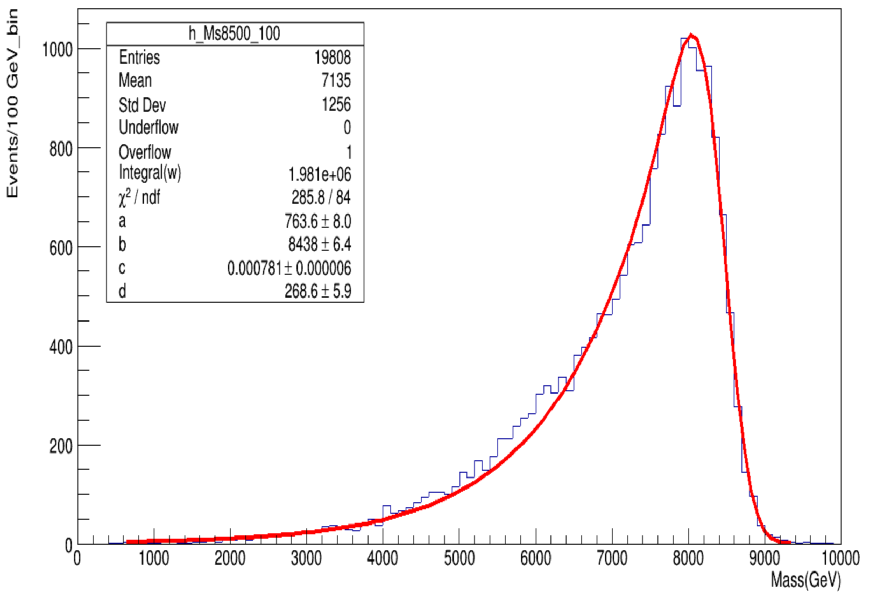
\includegraphics[width=0.45\textwidth]{figures/app-StrMorphShapeStudies/GcEFit_Old_ntuples_8p5TeV.png} }
  \subfigure[$M_{s} = 8.5$ TeV w/ GrL.]{
  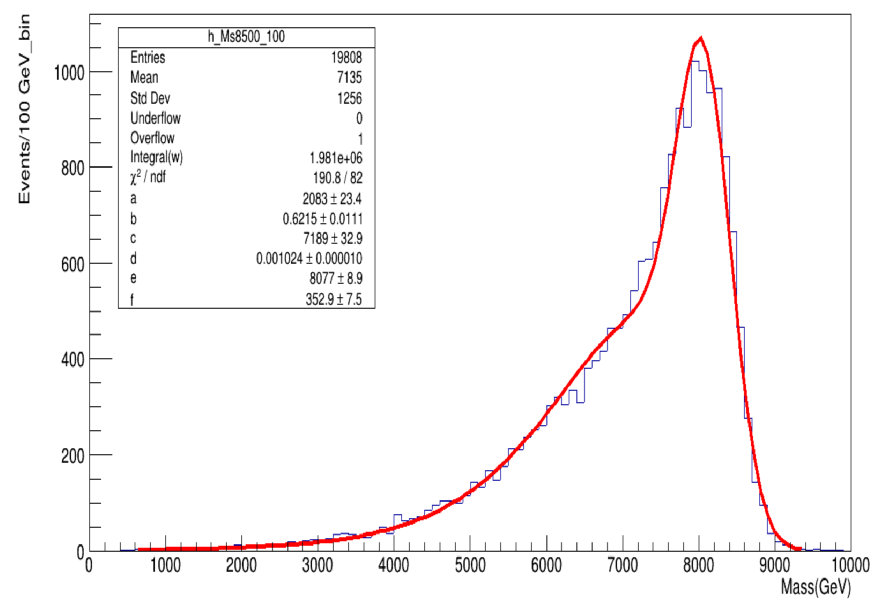
\includegraphics[width=0.45\textwidth]{figures/app-StrMorphShapeStudies/GrLFit_Old_ntuples_8p5TeV.png} }
  \subfigure[$M_{s} = 9.0$ TeV w/ GcE.]{
  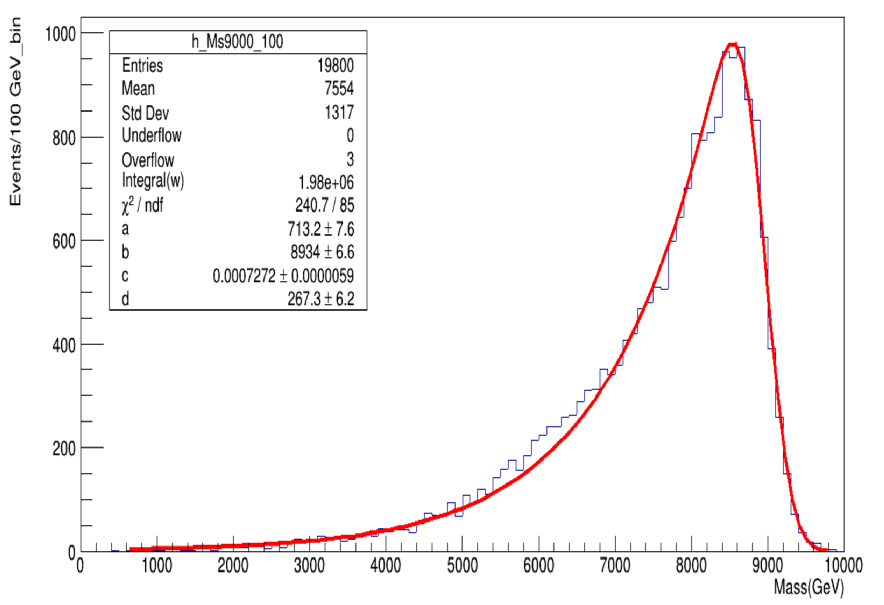
\includegraphics[width=0.45\textwidth]{figures/app-StrMorphShapeStudies/GcEFit_Old_ntuples_9TeV.png} }
  \subfigure[$M_{s} = 9.0$ TeV w/ GrL.]{
  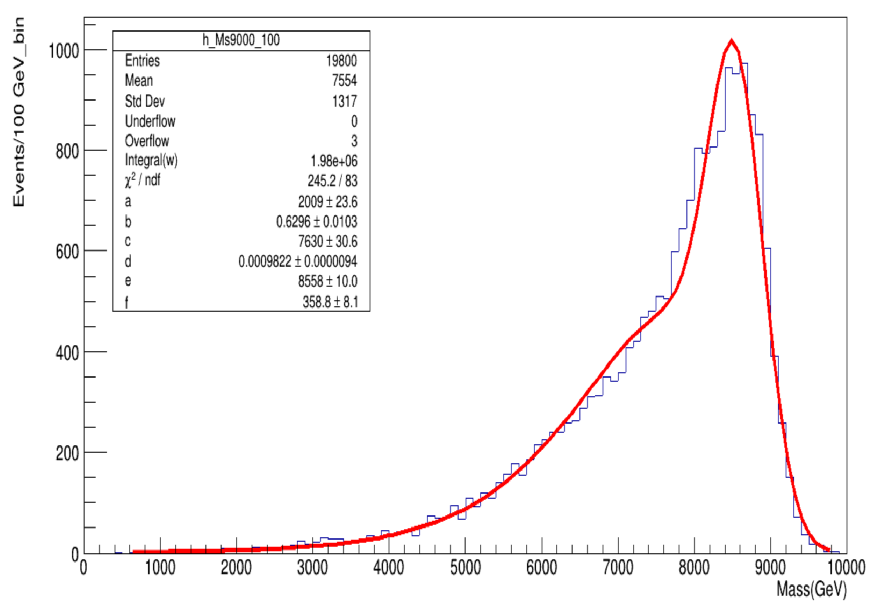
\includegraphics[width=0.45\textwidth]{figures/app-StrMorphShapeStudies/GrLFit_Old_ntuples_9TeV.png} }    
  \caption{The GcE and GrL fits on the string signal shapes for $M_{s} = 8.5$ and $9.0$ TeV.}
  \label{fig:InitGcEGrL-2}
\end{figure}

\clearpage

In order to have a better idea about the behaviour of the resultant fit parameters, they have been fitted with linear functions. Figures \ref{fig:InitGcEParam} and \ref{fig:InitGrLParam} contain the parameter-fits from the GcE and GrL fits respectively.  

\begin{figure}[!htb]
  \centering
  \subfigure[GcE: $a$ -- amplitude.]{
  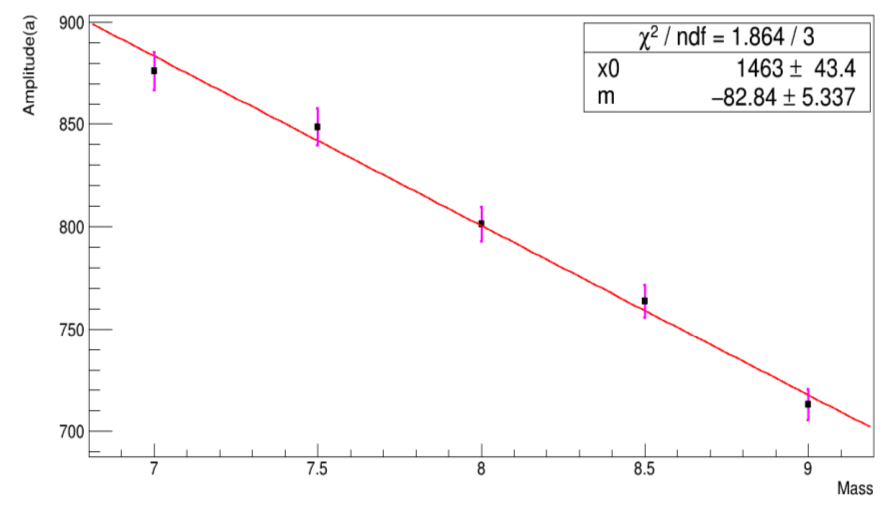
\includegraphics[width=0.45\textwidth]{figures/app-StrMorphShapeStudies/GcEFitParam_a_Old_ntuples.png} }
  \subfigure[GcE: $b$ -- Gaussian mean (offset).]{
  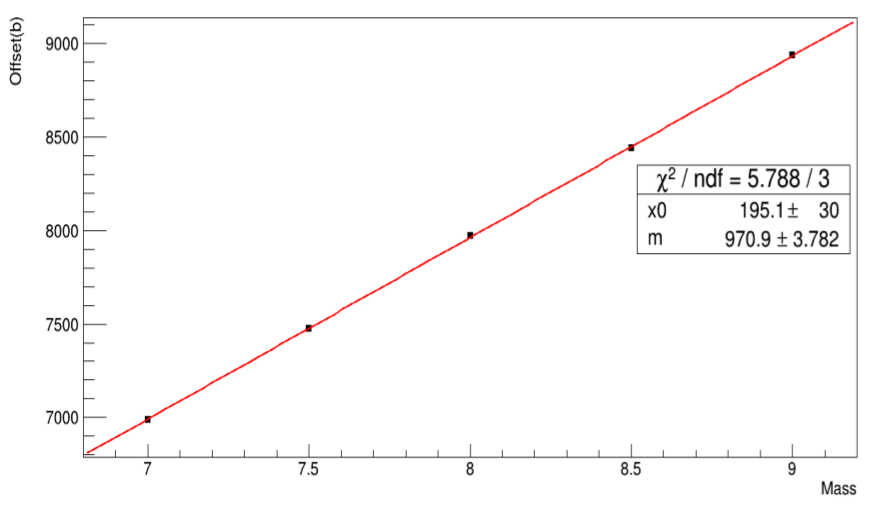
\includegraphics[width=0.45\textwidth]{figures/app-StrMorphShapeStudies/GcEFitParam_b_Old_ntuples.png} }
  \subfigure[GcE: $c$ -- lambda of exponential.]{
  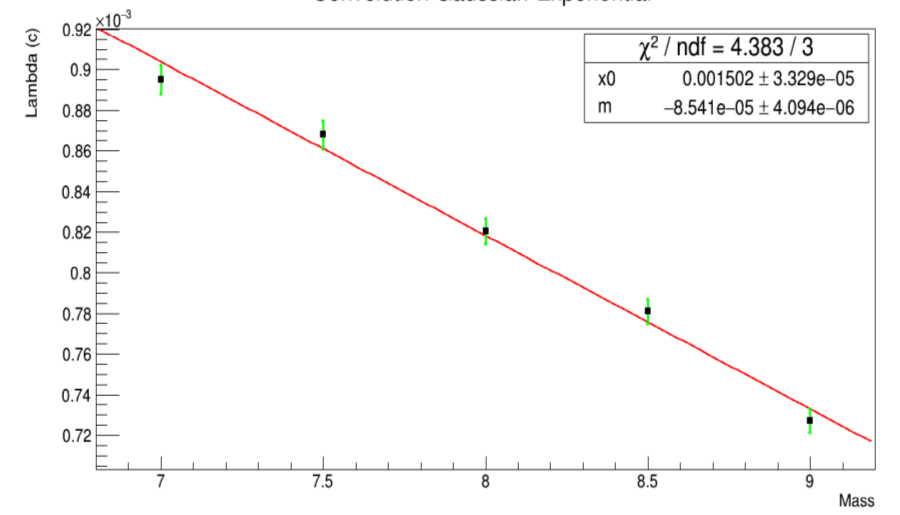
\includegraphics[width=0.45\textwidth]{figures/app-StrMorphShapeStudies/GcEFitParam_c_Old_ntuples.png} }
  \subfigure[GcE: $d$ -- Gaussian width (sigma).]{
  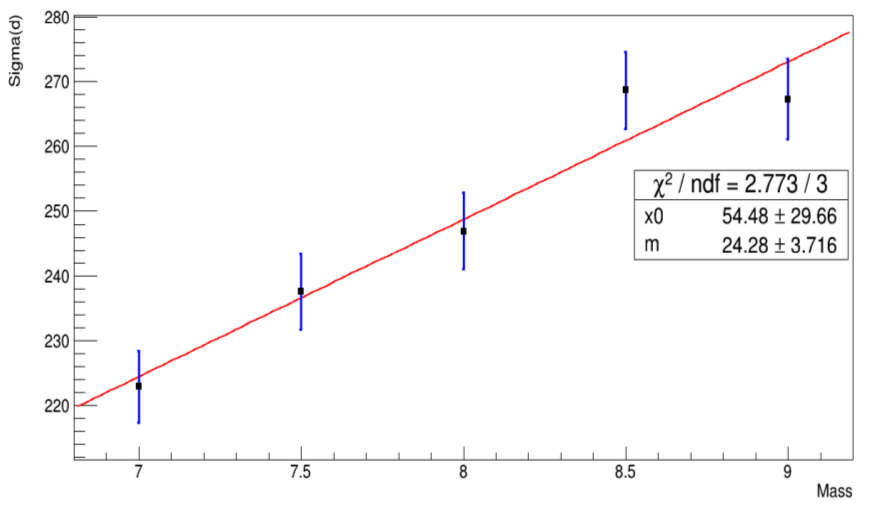
\includegraphics[width=0.45\textwidth]{figures/app-StrMorphShapeStudies/GcEFitParam_d_Old_ntuples.png} }
  \caption{The linearly fitted GcE fit parameters for $M_{s} = 7.0,~7.5,~8.0,~8.5$ and $9.0$ TeV.}
  \label{fig:InitGcEParam}
\end{figure}

\clearpage


\begin{figure}[!htb]
  \centering
  \subfigure[GrL: $a$ -- relative normalization.]{
  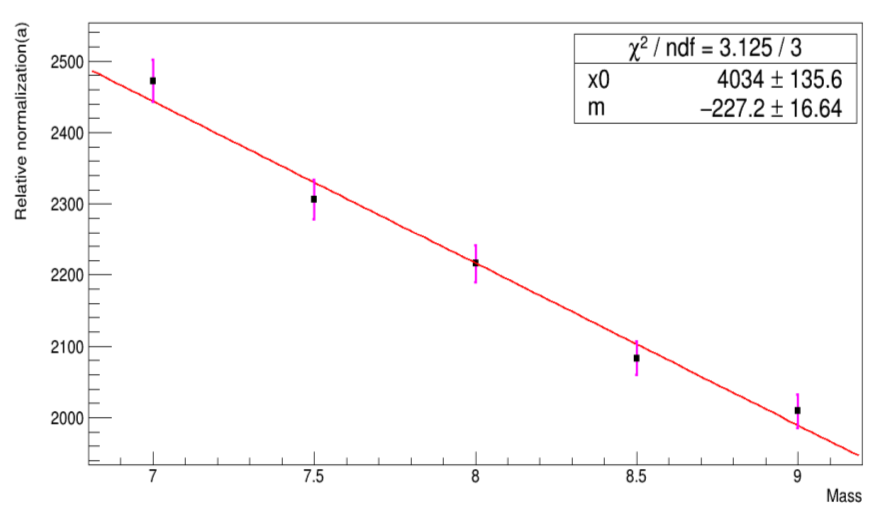
\includegraphics[width=0.45\textwidth]{figures/app-StrMorphShapeStudies/GrLFitParam_a_Old_ntuples.png} }
  \subfigure[GrL: $b$ -- fraction of reverse-Landau/Gaussian components.]{
  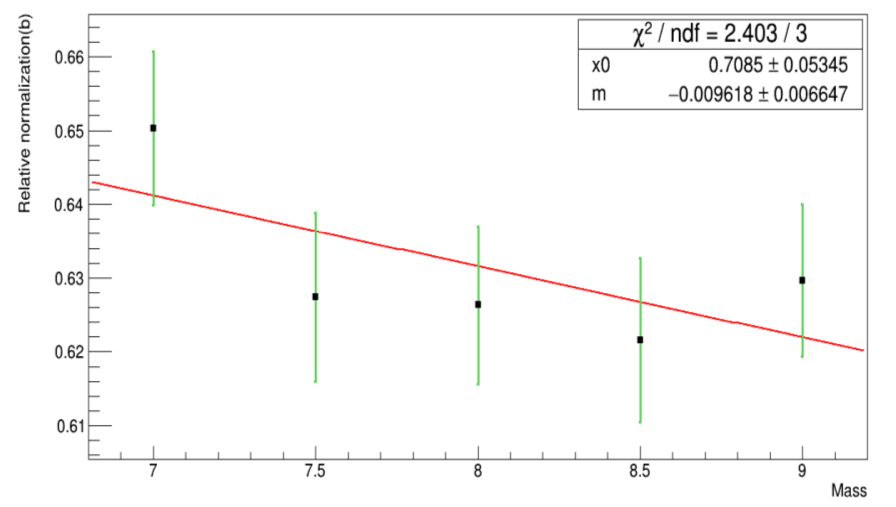
\includegraphics[width=0.45\textwidth]{figures/app-StrMorphShapeStudies/GrLFitParam_b_Old_ntuples.png} }
  \subfigure[GrL: $c$ -- reverse-Landau mean (offset).]{
  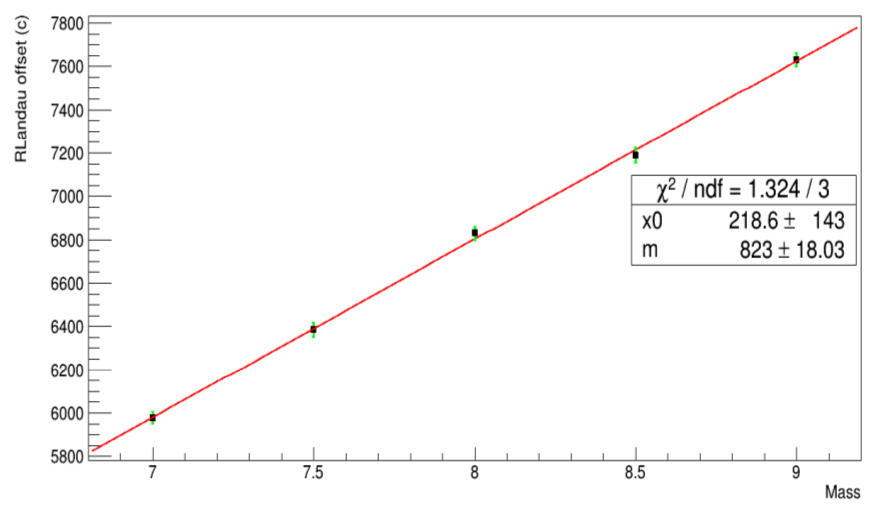
\includegraphics[width=0.45\textwidth]{figures/app-StrMorphShapeStudies/GrLFitParam_c_Old_ntuples.png} }
  \subfigure[GrL: $d$ -- reverse-Landau width (scale).]{
  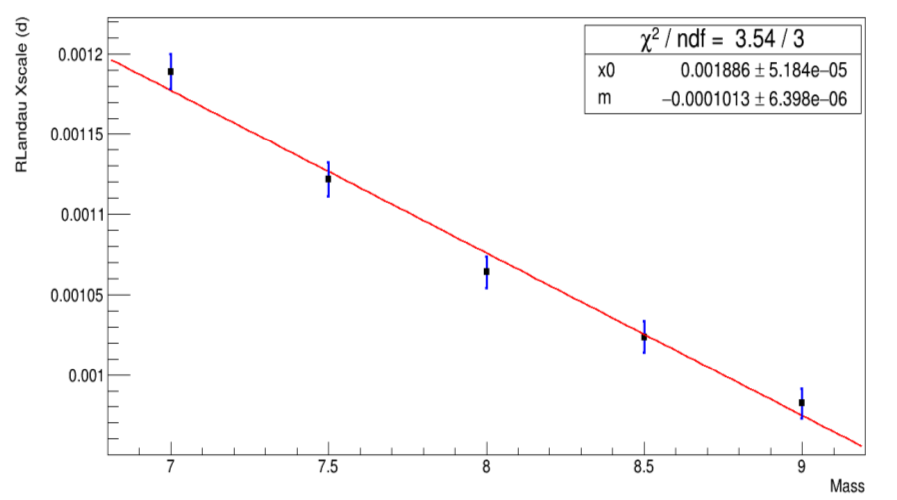
\includegraphics[width=0.45\textwidth]{figures/app-StrMorphShapeStudies/GrLFitParam_d_Old_ntuples.png} }
  \subfigure[GrL: $e$ -- Gaussian mean (offset).]{
  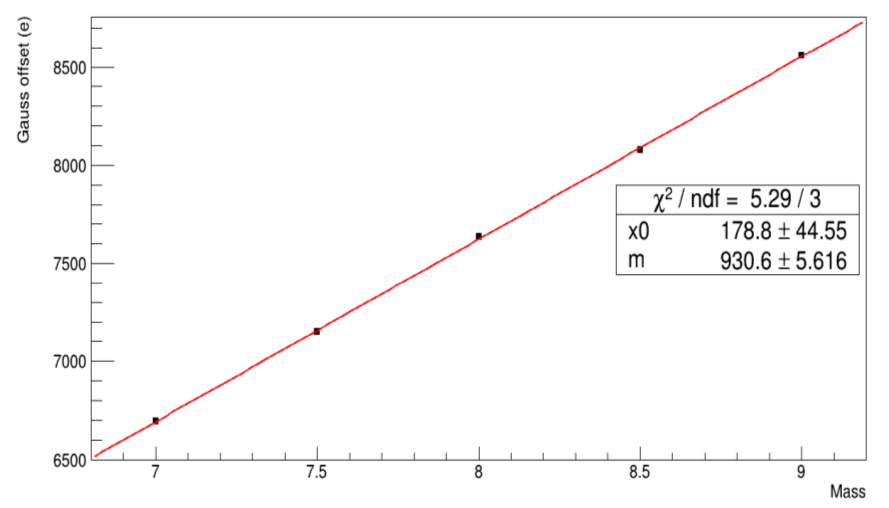
\includegraphics[width=0.45\textwidth]{figures/app-StrMorphShapeStudies/GrLFitParam_e_Old_ntuples.png} }
  \subfigure[GrL: $f$ -- Gaussian width (sigma).]{
  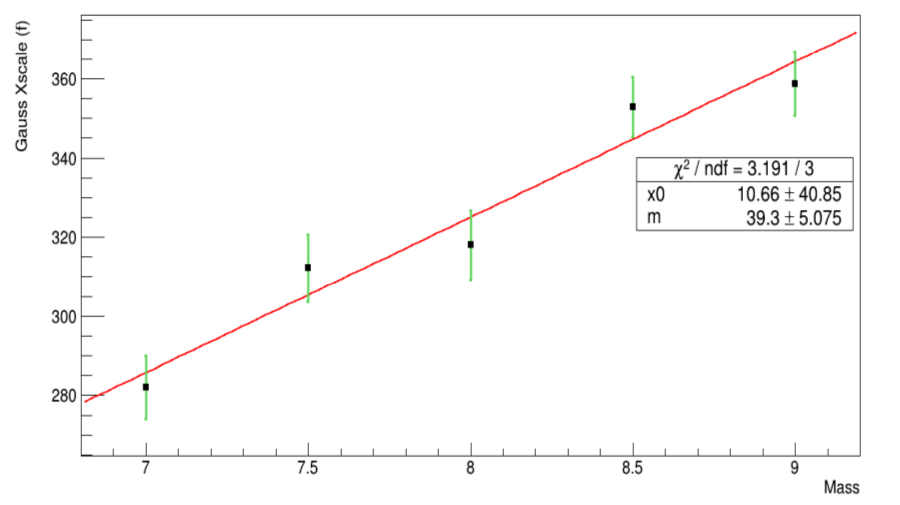
\includegraphics[width=0.45\textwidth]{figures/app-StrMorphShapeStudies/GrLFitParam_f_Old_ntuples.png} }
  \caption{The linearly fitted GrL fit parameters for $M_{s} = 7.0,~7.5,~8.0,~8.5$ and $9.0$ TeV.}
  \label{fig:InitGrLParam}
\end{figure}


The Figures \ref{fig:InitGcEGrL-1} and \ref{fig:InitGcEGrL-2} show that the individual GcE fits have better quality (the $\chi^2/\mathrm{ndf}$ values) than the corresponding GrL ones. On top of it, the linear behaviour of the fit parameters is also there for almost all the parameters (via Figures \ref{fig:InitGcEParam} and \ref{fig:InitGrLParam}) for GcE in comparison to GrL. From these two points, it could be concluded that GcE fits the string signal shape better than the conventional GrL. 
 
%-------------------------------------------------------------------------------

\subsection{Recent shape studies}
\label{subsec:StrMorphShapeStudies:ReceShapStud}
The findings from \ref{subsec:StrMorphShapeStudies:InitShapStud} are reused after the finalization of the selection cuts for the inclusive string analysis. The $m_{jj}$ string signal distributions are produced with $|\Delta\phi_{jj}|>1.0$, $|y^*|<0.8$ and $m_{jj}>1200$ GeV. Also, instead of the uniform $m_{jj}$ binning of 100 GeV, variable bin sizes with the following lower and upper limits are used -- \\

946, 976, 1006, 1037, 1068, 1100, 1133, 1166, 1200, 1234, 1269, 1305, 1341, 1378, 1416, 1454, 1493, 1533, 1573,1614, 1656, 1698, 1741, 1785, 1830, 1875, 1921, 1968, 2016, 2065, 2114, 2164, 2215, 2267, 2320, 2374, 2429, 2485, 2542, 2600, 2659, 2719, 2780, 2842, 2905, 2969, 3034, 3100, 3167, 3235, 3305, 3376, 3448, 3521, 3596, 3672, 3749, 3827, 3907, 3988, 4070, 4154, 4239, 4326, 4414, 4504, 4595, 4688, 4782, 4878, 4975, 5074, 5175, 5277, 5381, 5487, 5595, 5705, 5817, 5931, 6047, 6165, 6285, 6407, 6531, 6658, 6787, 6918, 7052, 7188, 7326, 7467, 7610, 7756, 7904, 8055, 8208, 8364, 8523, 8685, 8850, 9019, 9191, 9366, 9544, 9726, 9911, 10100, 10292, 10488, 10688, 10892, 11100, 11312, 11528, 11748, 11972, 12200, 12432, 12669, 12910, 13156 GeV.
   
~~~~~ Figure \ref{fig:ReceStrmjj} consists of the string signal shapes with selection cuts and binning described above. All these shapes are fitted with GcE, and after successful fits, the corresponding fit parameters are fitted using the cubic splines. As mentioned in the beginning, these cubic splines could be used for producing intermediate string signal shapes if needed. The GcE fits and the cubic splines are placed at Figures \ref{fig:ReceGcE} and \ref{fig:ReceGcEParam} respectively. 

\clearpage

\begin{figure}[!htb]
  \centering
  \subfigure[$M_{s} = 7.0$ TeV.]{
  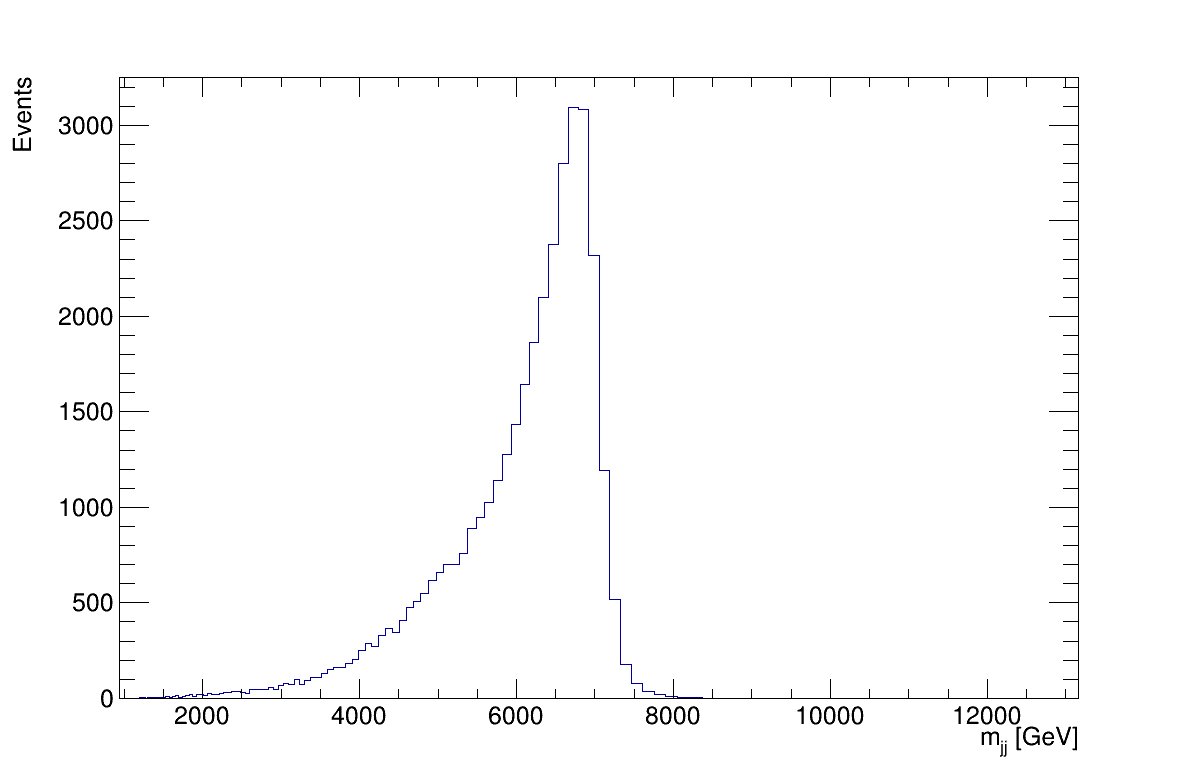
\includegraphics[width=0.45\textwidth]{figures/app-StrMorphShapeStudies/mjj_New_string_ntuples_7TeV.png} }
  \subfigure[$M_{s} = 7.5$ TeV.]{
  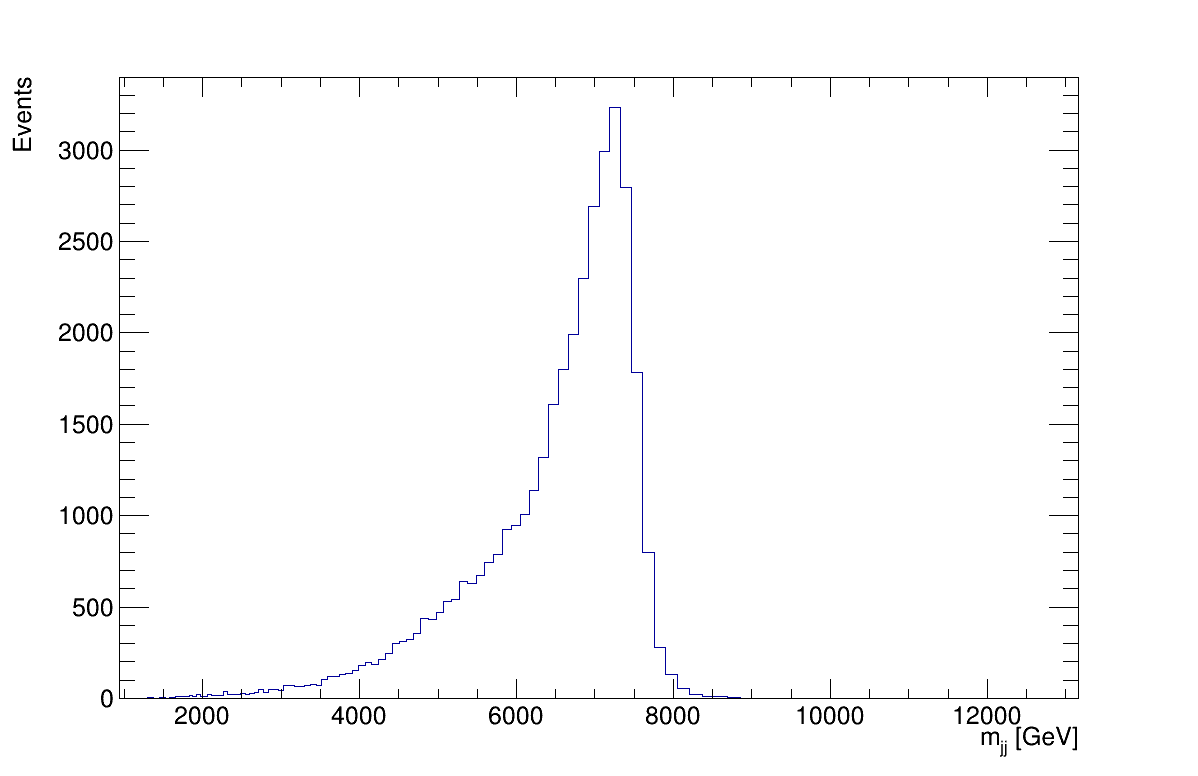
\includegraphics[width=0.45\textwidth]{figures/app-StrMorphShapeStudies/mjj_New_string_ntuples_7p5TeV.png} }
  \subfigure[$M_{s} = 8.0$ TeV.]{
  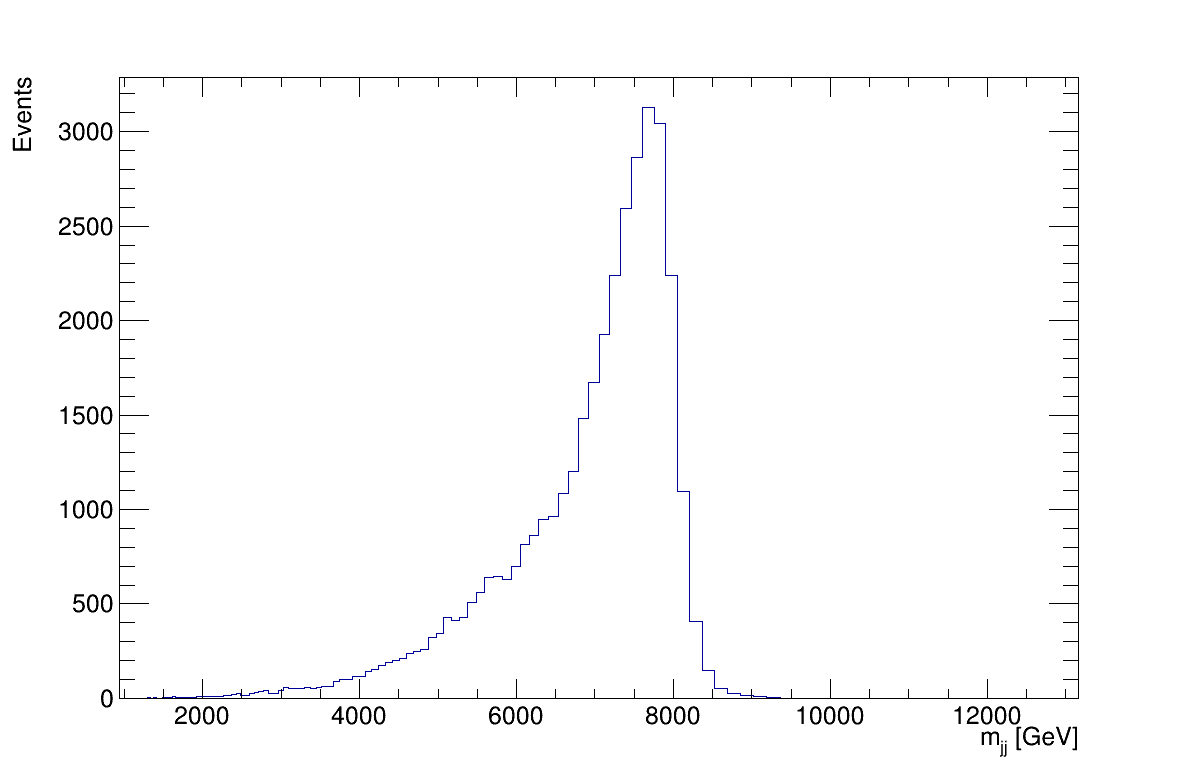
\includegraphics[width=0.45\textwidth]{figures/app-StrMorphShapeStudies/mjj_New_string_ntuples_8TeV.png} }
  \subfigure[$M_{s} = 8.5$ TeV.]{
  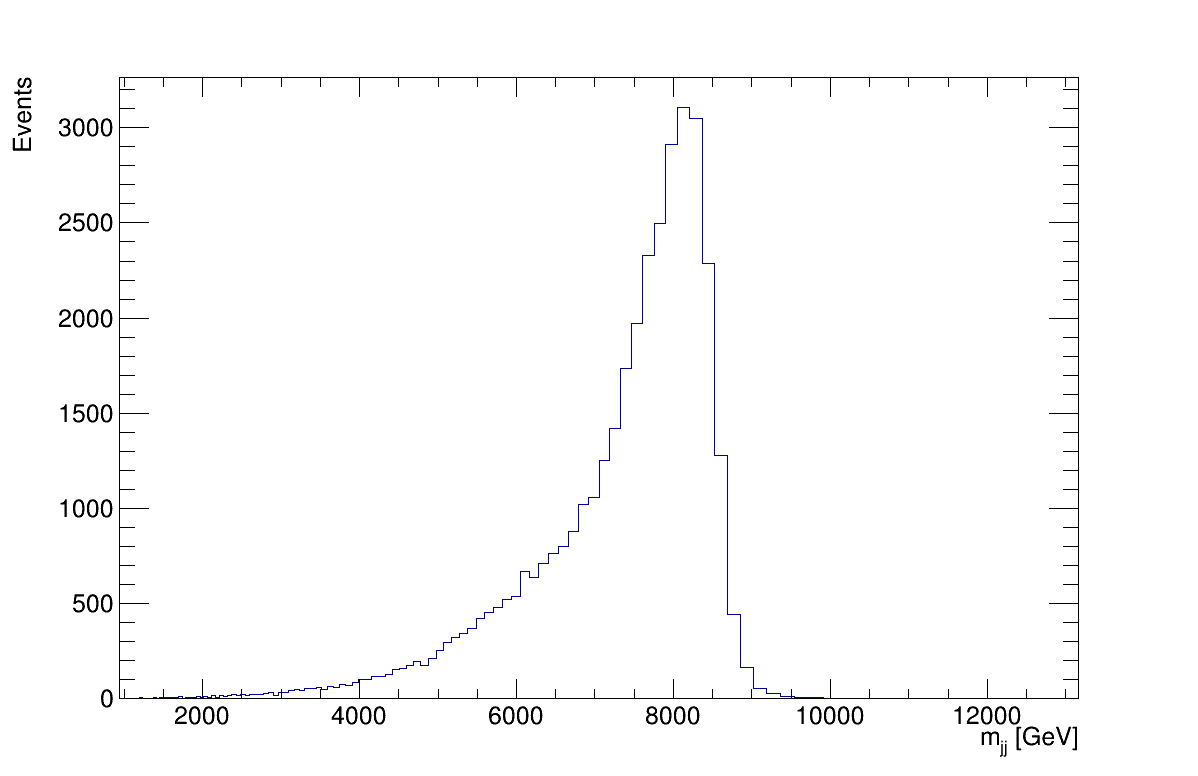
\includegraphics[width=0.45\textwidth]{figures/app-StrMorphShapeStudies/mjj_New_string_ntuples_8p5TeV.png} }
  \subfigure[$M_{s} = 9.0$ TeV.]{
  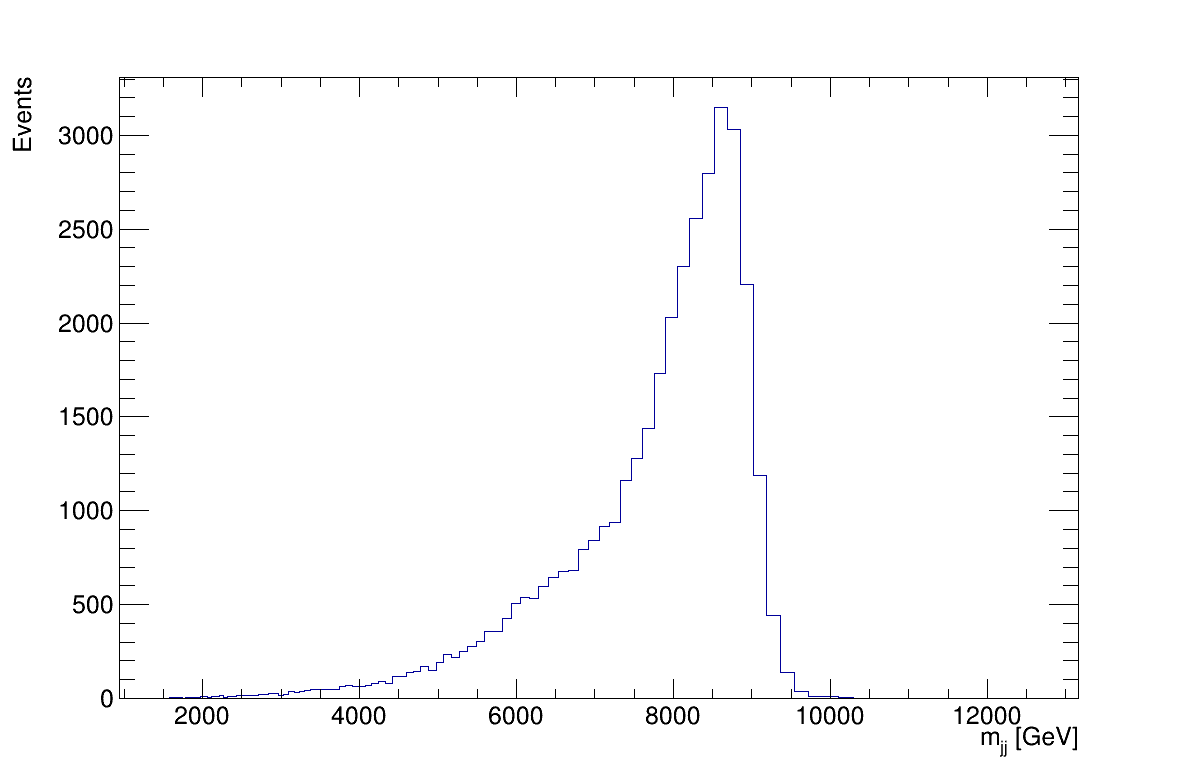
\includegraphics[width=0.45\textwidth]{figures/app-StrMorphShapeStudies/mjj_New_string_ntuples_9TeV.png} }
  \caption{The string signal $m_{jj}$ shapes from the corresponding MC samples with the selection cuts and variable binning.}
  \label{fig:ReceStrmjj}
\end{figure}

\clearpage

\begin{figure}[!htb]
  \centering
  \subfigure[GcE fit on $M_{s} = 7.0$ TeV (w/ selection cuts and variable binning).]{
  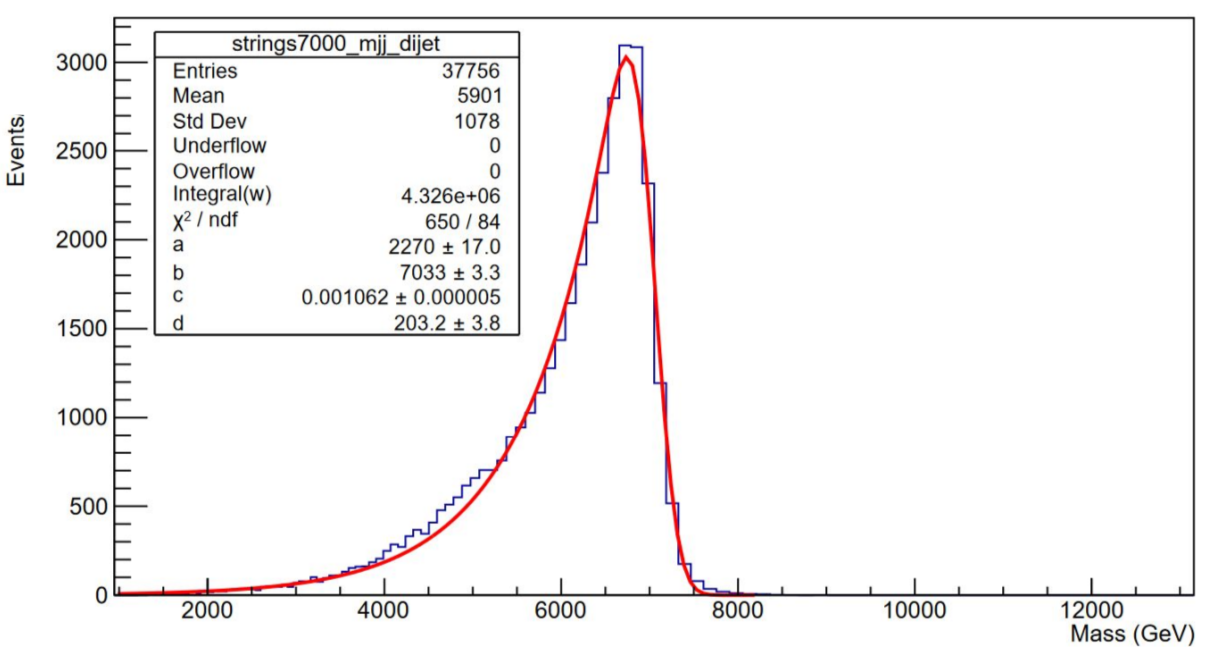
\includegraphics[width=0.45\textwidth]{figures/app-StrMorphShapeStudies/GcEFit_New_ntuples_7TeV.png} }
  \subfigure[GcE fit on $M_{s} = 7.5$ TeV (w/ selection cuts and variable binning).]{
  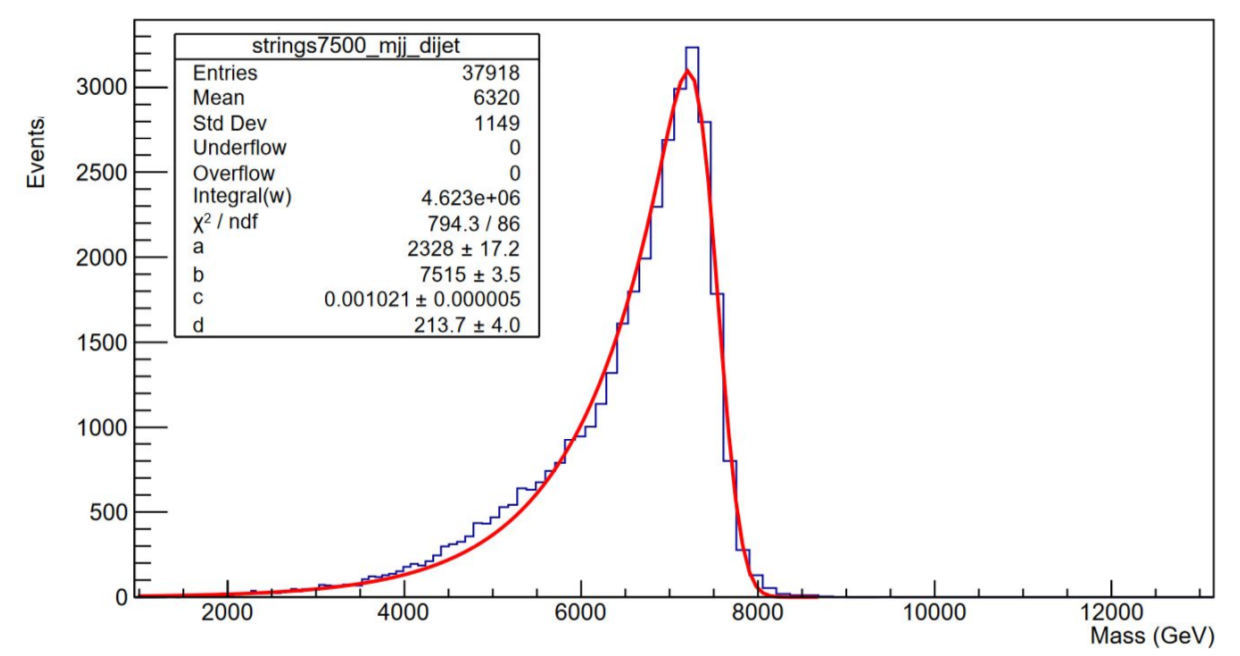
\includegraphics[width=0.45\textwidth]{figures/app-StrMorphShapeStudies/GcEFit_New_ntuples_7p5TeV.png} }
  \subfigure[GcE fit on $M_{s} = 8.0$ TeV (w/ selection cuts and variable binning).]{
  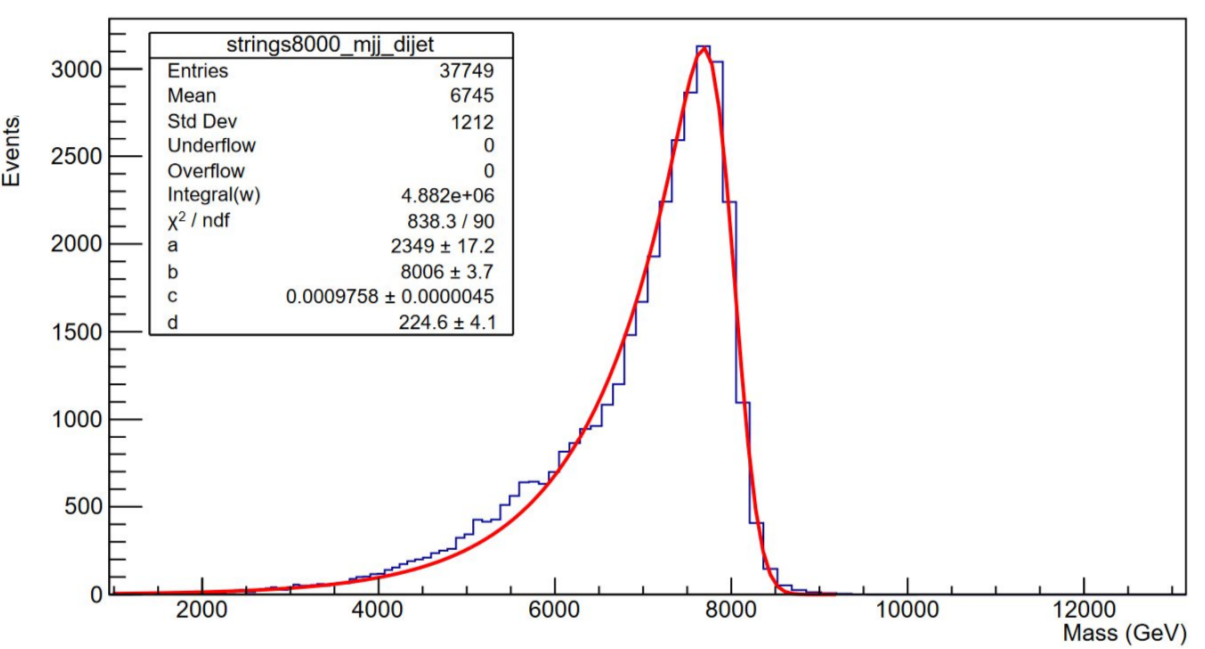
\includegraphics[width=0.45\textwidth]{figures/app-StrMorphShapeStudies/GcEFit_New_ntuples_8TeV.png} }
  \subfigure[GcE fit on $M_{s} = 8.5$ TeV (w/ selection cuts and variable binning).]{
  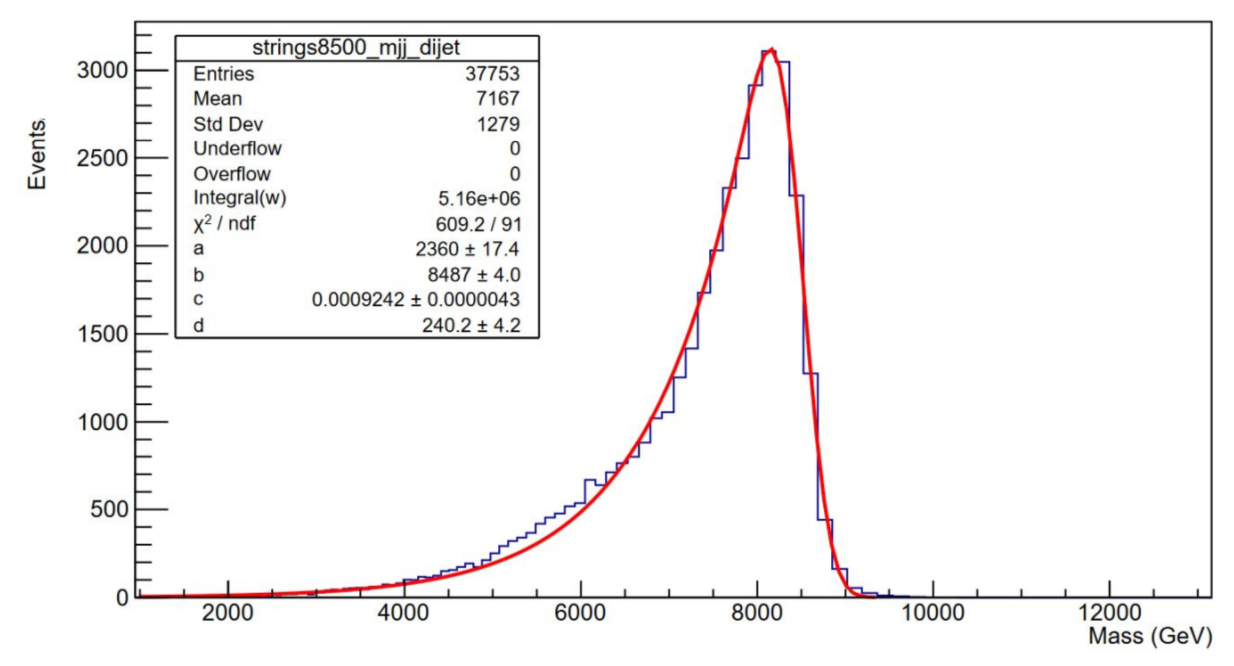
\includegraphics[width=0.45\textwidth]{figures/app-StrMorphShapeStudies/GcEFit_New_ntuples_8p5TeV.png} }
  \subfigure[GcE fit on $M_{s} = 9.0$ TeV (w/ selection cuts and variable binning).]{
  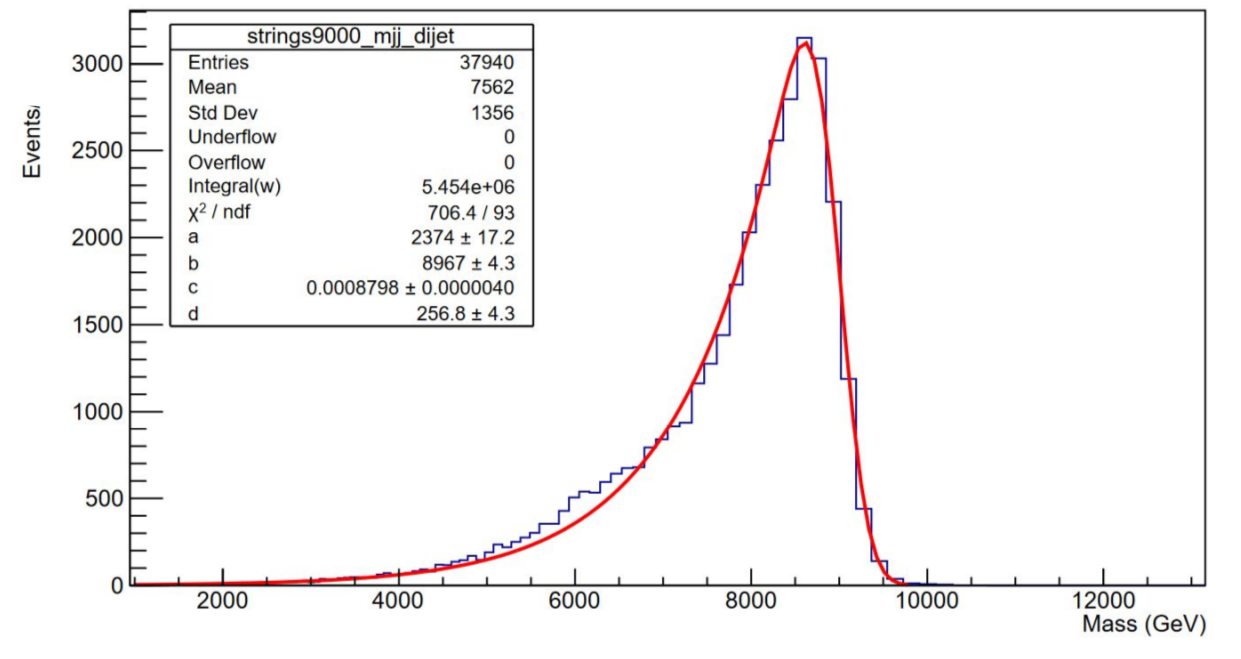
\includegraphics[width=0.45\textwidth]{figures/app-StrMorphShapeStudies/GcEFit_New_ntuples_9TeV.png} }
  \caption{GcE fits for string signal shapes after cuts and variable binning.}
  \label{fig:ReceGcE}
\end{figure}

\clearpage

\begin{figure}[!htb]
  \centering
  \subfigure[GcE: $a$ -- amplitude.]{
  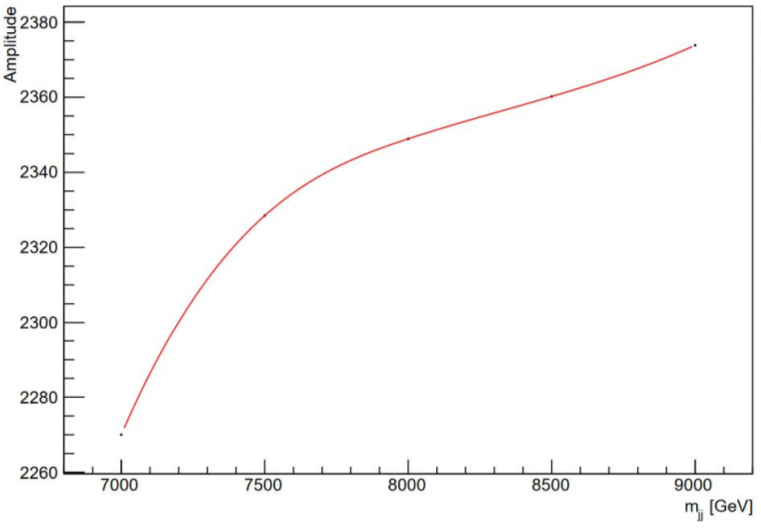
\includegraphics[width=0.45\textwidth]{figures/app-StrMorphShapeStudies/GcEFitParam_a_New_ntuples.png} }
  \subfigure[GcE: $b$ -- Gaussian mean (offset).]{
  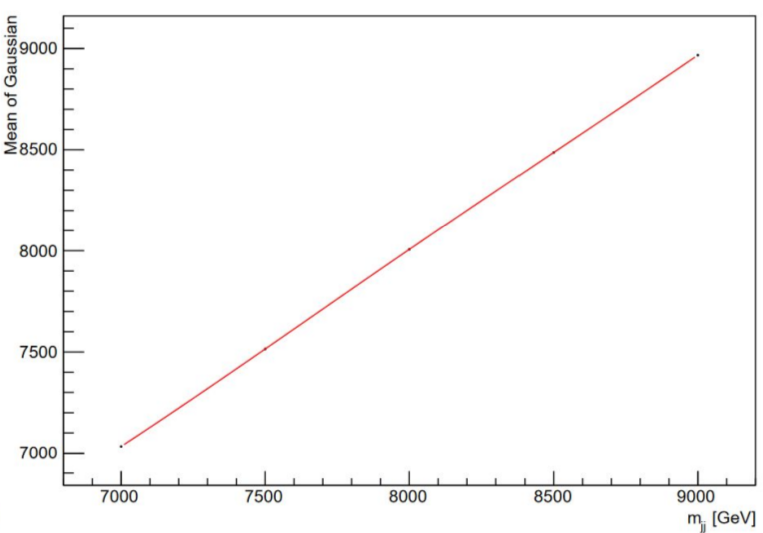
\includegraphics[width=0.45\textwidth]{figures/app-StrMorphShapeStudies/GcEFitParam_b_New_ntuples.png} }
  \subfigure[GcE: $c$ -- lambda of exponential.]{
  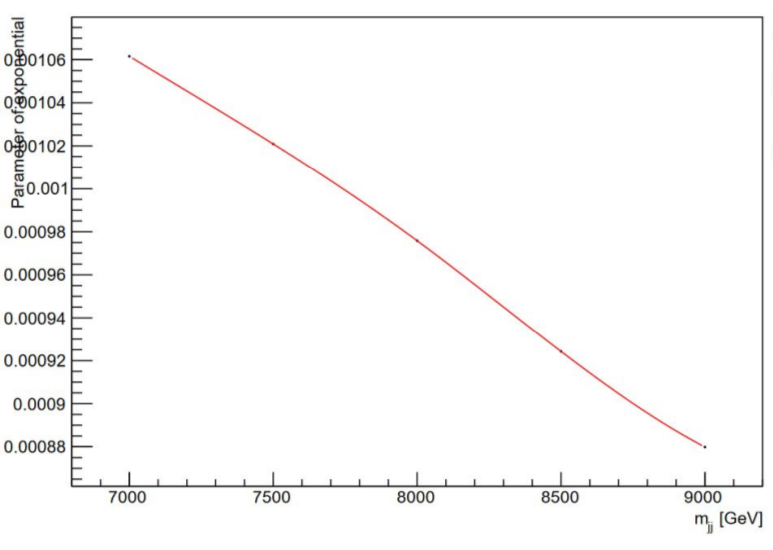
\includegraphics[width=0.45\textwidth]{figures/app-StrMorphShapeStudies/GcEFitParam_c_New_ntuples.png} }
  \subfigure[GcE: $d$ -- Gaussian width (sigma).]{
  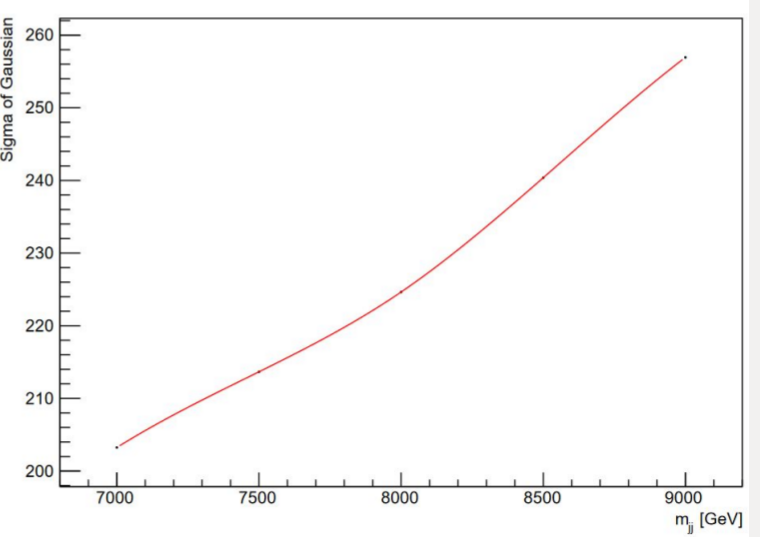
\includegraphics[width=0.45\textwidth]{figures/app-StrMorphShapeStudies/GcEFitParam_d_New_ntuples.png} }
  \caption{The cubic splines of GcE fit parameters for $M_{s} = 7.0,~7.5,~8.0,~8.5$ and $9.0$ TeV (after selection cuts and variable binning).}
  \label{fig:ReceGcEParam}
\end{figure}


%-------------------------------------------------------------------------------

\subsection{Summary}
\label{subsec:StrMorphShapeStudies:Summary}
The shape studies of the string signal MC samples with various fit functions lead to the conclusion that the convolution between a Gaussian and an exponential (GcE) is the best suited template for them. 


%-------------------------------------------------------------------------------
